% Copyright 2006 by Till Tantau
%
% This file may be distributed and/or modified
%
% 1. under the LaTeX Project Public License and/or
% 2. under the GNU Free Documentation License.
%
% See the file doc/generic/pgf/licenses/LICENSE for more details.


\section{Design Principles}

This section describes the design principles behind the \tikzname\ frontend,
where \tikzname\ means ``\tikzname\ ist \emph{kein} Zeichenprogramm''. To use
\tikzname, as a \LaTeX\ user say |\usepackage{tikz}| somewhere in the preamble,
as a plain \TeX\ user say |\input tikz.tex|. \tikzname's job is to make your
life easier by providing an easy-to-learn and easy-to-use syntax for describing
graphics.

The commands and syntax of \tikzname\ were influenced by several sources. The
basic command names and the notion of path operations is taken from
\textsc{metafont}, the option mechanism comes from \textsc{pstricks}, the
notion of styles is reminiscent of \textsc{svg}, the graph syntax is taken from
\textsc{graphviz}. To make it all work together, some compromises were
necessary. I also added some ideas of my own, like coordinate transformations.

The following basic design principles underlie \tikzname:
%
\begin{enumerate}
    \item Special syntax for specifying points.
    \item Special syntax for path specifications.
    \item Actions on paths.
    \item Key--value syntax for graphic parameters.
    \item Special syntax for nodes.
    \item Special syntax for trees.
    \item Special syntax for graphs.
    \item Grouping of graphic parameters.
    \item Coordinate transformation system.
\end{enumerate}


\subsection{Special Syntax For Specifying Points}

\tikzname\ provides a special syntax for specifying points and coordinates. In
the simplest case, you provide two \TeX\ dimensions, separated by commas, in
round brackets as in |(1cm,2pt)|.

You can also specify a point in polar coordinates by using a colon instead of a
comma as in |(30:1cm)|, which means ``1cm in a 30 degrees direction''.

If you do not provide a unit, as in |(2,1)|, you specify a point in \pgfname's
$xy$-coordinate system. By default, the unit $x$-vector goes 1cm to the right
and the unit $y$-vector goes 1cm upward.

By specifying three numbers as in |(1,1,1)| you specify a point in \pgfname's
$xyz$-coordinate system.

It is also possible to use an anchor of a previously defined shape as in
|(first node.south)|.

You can add two plus signs before a coordinate as in |++(1cm,0pt)|. This means
``1cm to the right of the last point used''. This allows you to easily specify
relative movements. For example, |(1,0) ++(1,0) ++(0,1)| specifies the three
coordinates |(1,0)|, then |(2,0)|, and |(2,1)|.

Finally, instead of two plus signs, you can also add a single one. This also
specifies a point in a relative manner, but it does not ``change'' the current
point used in subsequent relative commands. For example, |(1,0) +(1,0) +(0,1)|
specifies the three coordinates |(1,0)|, then |(2,0)|, and |(1,1)|.


\subsection{Special Syntax For Path Specifications}

When creating a picture using \tikzname, your main job is the specification of
\emph{paths}. A path is a series of straight or curved lines, which need not be
connected. \tikzname\ makes it easy to specify paths, partly using the syntax
of \textsc{metapost}. For example, to specify a triangular path you use
%
\begin{codeexample}[code only]
(5pt,0pt) -- (0pt,0pt) -- (0pt,5pt) -- cycle
\end{codeexample}
%
and you get \tikz \draw (5pt,0pt) -- (0pt,0pt) -- (0pt,5pt) -- cycle; when you
draw this path.


\subsection{Actions on Paths}

A path is just a series of straight and curved lines, but it is not yet
specified what should happen with it. One can \emph{draw} a path, \emph{fill} a
path, \emph{shade} it, \emph{clip} it, or do any combination of these. Drawing
(also known as \emph{stroking}) can be thought of as taking a pen of a certain
thickness and moving it along the path, thereby drawing on the canvas. Filling
means that the interior of the path is filled with a uniform color. Obviously,
filling makes sense only for \emph{closed} paths and a path is automatically
closed prior to filling, if necessary.

Given a path as in |\path (0,0) rectangle (2ex,1ex);|, you can draw it by
adding the |draw| option as in |\path[draw] (0,0) rectangle (2ex,1ex);|, which
yields \tikz \path[draw] (0,0) rectangle (2ex,1ex);. The |\draw| command is
just an abbreviation for |\path[draw]|. To fill a path, use the |fill| option
or the |\fill| command, which is an abbreviation for |\path[fill]|. The
|\filldraw| command is an abbreviation for |\path[fill,draw]|. Shading is
caused by the |shade| option (there are |\shade| and |\shadedraw|
abbreviations) and clipping by the |clip| option. There is also a |\clip|
command, which does the same as |\path[clip]|, but not commands like
|\drawclip|. Use, say, |\draw[clip]| or |\path[draw,clip]| instead.

All of these commands can only be used inside |{tikzpicture}| environments.

\tikzname\ allows you to use different colors for filling and stroking.


\subsection{Key--Value Syntax for Graphic Parameters}

Whenever \tikzname\ draws or fills a path, a large number of graphic parameters
influences the rendering. Examples include the colors used, the dashing
pattern, the clipping area, the line width, and many others. In \tikzname, all
these options are specified as lists of so called key--value pairs, as in
|color=red|, that are passed as optional parameters to the path drawing and
filling commands. This usage is similar to \textsc{pstricks}. For example, the
following will draw a thick, red triangle;
%
\begin{codeexample}[]
\tikz \draw[line width=2pt,color=red] (1,0) -- (0,0) -- (0,1) -- cycle;
\end{codeexample}


\subsection{Special Syntax for Specifying Nodes}

\tikzname\ introduces a special syntax for adding text or, more generally,
nodes to a graphic. When you specify a path, add nodes as in the following
example:
%
\begin{codeexample}[]
\tikz \draw (1,1) node {text} -- (2,2);
\end{codeexample}
%
Nodes are inserted at the current position of the path, but either \emph{after}
(the default) or \emph{before} the complete path is rendered. When special
options are given, as in |\draw (1,1) node[circle,draw] {text};|, the text is
not just put at the current position. Rather, it is surrounded by a circle and
this circle is ``drawn''.

You can add a name to a node for later reference either by using the option
|name=|\meta{node name} or by stating the node name in parentheses outside the
text as in |node[circle](name){text}|.

Predefined shapes include |rectangle|, |circle|, and |ellipse|, but it is
possible (though a bit challenging) to define new shapes.


\subsection{Special Syntax for Specifying Trees}

The ``node syntax'' can also be used to draw tress: A |node| can be followed by
any number of children, each introduced by the keyword |child|. The children
are nodes themselves, each of which may have children in turn.
%
\begin{codeexample}[]
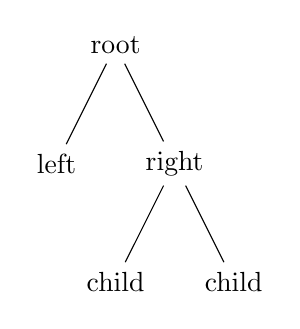
\begin{tikzpicture}
  \node {root}
    child {node {left}}
    child {node {right}
      child {node {child}}
      child {node {child}}
    };
\end{tikzpicture}
\end{codeexample}
%
Since trees are made up from nodes, it is possible to use options to modify the
way trees are drawn. Here are two examples of the above tree, redrawn with
different options:
%
\begin{codeexample}[preamble={\usetikzlibrary{arrows,trees}}]
\begin{tikzpicture}
  [edge from parent fork down, sibling distance=15mm, level distance=15mm,
   every node/.style={fill=red!30,rounded corners},
   edge from parent/.style={red,-o,thick,draw}]
  \node {root}
      child {node {left}}
      child {node {right}
        child {node {child}}
        child {node {child}}
      };
\end{tikzpicture}
\end{codeexample}

\begin{codeexample}[]
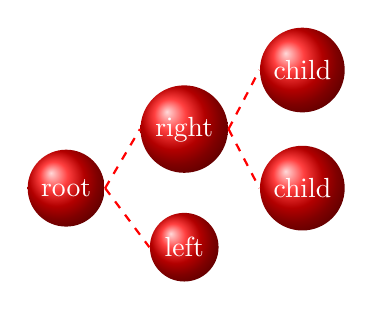
\begin{tikzpicture}
  [parent anchor=east,child anchor=west,grow=east,
   sibling distance=15mm, level distance=15mm,
   every node/.style={ball color=red,circle,text=white},
   edge from parent/.style={draw,dashed,thick,red}]
  \node {root}
      child {node {left}}
      child {node {right}
        child {node {child}}
        child {node {child}}
      };
\end{tikzpicture}
\end{codeexample}


\subsection{Special Syntax for Graphs}

The |\node| command gives you fine control over where nodes should be placed,
what text they should use, and what they should look like. However, when you
draw a graph, you typically need to create numerous fairly similar nodes that
only differ with respect to the name they show. In these cases, the |graph|
syntax can be used, which is another syntax layer build ``on top'' of the node
syntax.
%
\begin{codeexample}[preamble={\usetikzlibrary{graphs}}]
\tikz \graph [grow down, branch right] {
  root -> { left, right -> {child, child} }
};
\end{codeexample}
%
The syntax of the |graph| command extends the so-called \textsc{dot}-notation
used in the popular \textsc{graphviz} program.

Depending on the version of \TeX\ you use (it must allow you to call Lua code,
which is the case for Lua\TeX), you can also ask \tikzname\ to do automatically
compute good positions for the nodes of a graph using one of several integrated
\emph{graph drawing algorithms}.


\subsection{Grouping of Graphic Parameters}

Graphic parameters should often apply to several path drawing or filling
commands. For example, we may wish to draw numerous lines all with the same
line width of 1pt. For this, we put these commands in a |{scope}| environment
that takes the desired graphic options as an optional parameter. Naturally, the
specified graphic parameters apply only to the drawing and filling commands
inside the environment. Furthermore, nested |{scope}| environments or
individual drawing commands can override the graphic parameters of outer
|{scope}| environments. In the following example, three red lines, two green
lines, and one blue line are drawn:
%
\begin{codeexample}[]
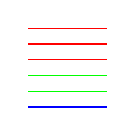
\begin{tikzpicture}
  \begin{scope}[color=red]
    \draw (0mm,10mm) -- (10mm,10mm);
    \draw (0mm, 8mm) -- (10mm, 8mm);
    \draw (0mm, 6mm) -- (10mm, 6mm);
  \end{scope}
  \begin{scope}[color=green]
    \draw             (0mm, 4mm) -- (10mm, 4mm);
    \draw             (0mm, 2mm) -- (10mm, 2mm);
    \draw[color=blue] (0mm, 0mm) -- (10mm, 0mm);
  \end{scope}
\end{tikzpicture}
\end{codeexample}

The |{tikzpicture}| environment itself also behaves like a |{scope}|
environment, that is, you can specify graphic parameters using an optional
argument. These optional apply to all commands in the picture.


\subsection{Coordinate Transformation System}

\tikzname\ supports both \pgfname's \emph{coordinate} transformation system to
perform transformations as well as \emph{canvas} transformations, a more
low-level transformation system. (For details on the difference between
coordinate transformations and canvas transformations see
Section~\ref{section-design-transformations}.)

The syntax is set up in such a way that it is harder to use canvas
transformations than coordinate transformations. There are two reasons for
this: First, the canvas transformation must be used with great care and often
results in ``bad'' graphics with changing line width and text in wrong sizes.
Second, \pgfname\ loses track of where nodes and shapes are positioned when
canvas transformations are used. So, in almost all circumstances, you should
use coordinate transformations rather than canvas transformations.
